\documentclass{article}
\usepackage[utf8]{inputenc}
\usepackage[T1]{fontenc}
\usepackage{graphicx}
\usepackage{float}
\begin{document}

\section*{Slide 1}

Prepared for submission to JINST

Topical Workshop on Electronics for Particle Physics - TWEPP2022 
19 - 23 September, 2022 
Bergen, Norway

Radiation studies performed on the High Luminosity 
ATLAS TileCal link Daughterboard

E. Valdes Santurio a, 1   , S. Silverstein a , C. Bohm a , H. Motzkau a , C. Clement a , K. 
Dunne a , S. Lee a on behalf of the ATLAS Tile Calorimeter System 2,3

a Stockholm University, Stockholm, Sweden

E-mail:   eduardo.valdes@fysik.su.se

Abstract:   The   new   electronics   of   the   ATLAS   Tile   Calorimeter   for   the   HL-LHC   interfaces   the 
on-detector   and   off-detector   electronics   by   means   of   a   Daughterboard. 
The   Daughterboard   is 
positioned   on-detector   featuring   commercial   SFPs+,   CERN   GBTx   ASICs,   ProASIC   FPGAs   and 
Kintex   Ultrascale   FPGAs.   The   design   minimizes   single   points   of   failure   and   mitigates   radiation 
damage   by   means   of   a   double   redundant   scheme,   Triple   Mode   Redundancy,   Xilinx   Soft   Error 
Mitigation   IP,   CRC/FEC   for   link   data   transfer,   and   SEL   protection   circuitry. 
We   present   an 
updated   summary   of   the   TID,   NIEL   and   SEE   qualification   tests,   and   performance   studies   of   the 
Daughterboard revision 6 design.

ATL-TILECAL-PROC-2022-017 
16 October 2022

Keywords:   Radiation damage to electronic components, Front-end electronics for detector readout.

1 Corresponding author. 
2 This work was supported by Stockholm University and CERN. 
3 Copyright 2020, CERN, for the benefit of the ATLAS Collaboration.   CC-BY-4.0 license.

\section*{Slide 2}

Contents

1 
Introduction 
1

2 
Tilecal read-out system for the HL-LHC 
2

3 
ATLAS TileCal link Daughterboard 
2

4 
Radiation tests on the DB6 
3

5 
Conclusions 
5

1 
Introduction

The Tile Calorimeter (TileCal) is a sampling calorimeter of the ATLAS Experiment [ 1 ].   TileCal is 
in charge of identifying and measuring hadronic jets and transverse missing energy.   As depicted in 
Figure  1 , the electronics for the read-out of all the TileCal are divided in four cylindrical barrels, each 
composed of 64 wedge-shaped modules where plastic scintillator tiles are used as active material 
interleaved   with   steel   plates   used   as   absorbers.   Light   from   two   sides   of   a   pseudo-projective   cell 
composed by a group of scintillators is collected by wavelength shifting fibers and read out by two 
photomultiplier tubes (PMTs).   To face the higher radiation levels and increased rates of pileup at 
the High Luminosity Large Hadron Collider (HL-LHC), the TileCal electronics will be upgraded 
with   a   new   design   that   will   provide   continuous   digital   read-out   of   all   the   TileCal   with   improved 
timing and better energy resolution.

\begin{figure}[H]
\centering
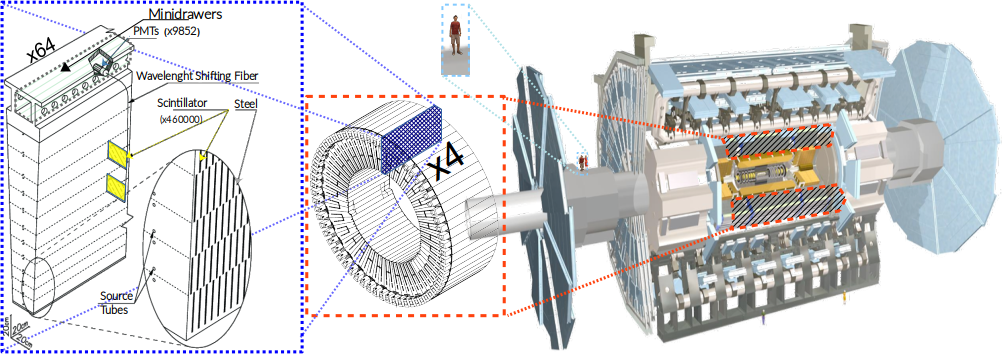
\includegraphics[width=0.8\linewidth]{assets/paper_ATL-TILECAL-PROC-2022-017_slide_2_item_1.png}
\end{figure}

Figure 1 .   TileCal structure in ATLAS.

-- 1 --

\section*{Slide 3}

2 
Tilecal read-out system for the HL-LHC

The off-detector electronics of the upgraded TileCal will provide digitized signals at 40 MHz to the 
Level 0 trigger system through the Trigger and Data Acquisition interface, while the so-called Front- 
End   Link   eXchange   (FELIX)   system   will   read-out   data   stored   in   pipelines   in   Tile   Preprocessors 
(TilePPr) at 1 MHz.   The TilePPrs will interface the on- and off-detector electronics through multi- 
Gbps   optical   links.   The   power   will   be   monitored   and   distributed   to   the   on-detector   electronics 
by the Detector Control System that interfaces with the Low Voltage Power Supplies in charge of 
distributing power to all the digital and analogue electronics, and the High Voltage Power Supplies 
that will provide high voltage to each PMT. 
The on-detector is comprised by 896 Minidrawers (MDs), in which data from all TileCal PMTs 
will continuously be sampled at 40 MHz.   Each MD will host up to twelve channels by means of 
twelve   PMTs   that   turn   light   pulses   to   electric   signals   to   be   shaped   and   conditioned   by   Front-End 
Boards.   A   Mainboard   (MB)   will   continuously   sample   and   digitize   two   gains   of   shaped   signals 
of   the   MD   PMTs.   A   Daughterboard   (DB)   is   in   charge   of   distributing   LHC   synchronized   timing, 
configuration and control to the front-end,   and continuously transmitting the digital data from all 
the MB channels to the off-detector systems via multi-Gbps optical links.

3 
ATLAS TileCal link Daughterboard

The DB is a radiation tolerant board with a redundancy layer of two functionally-equivalent halves, 
interconnecting   the   on-   and   off-detector   by   means   of   a   400-pin   FMC   connector   and   multi-Gbps 
optical links, respectively [ 3 ].   The DB, currently on its sixth revision (DB6, Figure  2 ), powers the 
optical links by means of four SFP+ modules that drive two downlinks and four uplinks.   The board 
information received by the board from the off-detector by means of 4.8 Gbps GBT-FEC downlinks 
powered   by   CERN   radiation   hard   GBTx   ASICs   includes   clock   signals,   time   synchronization   and 
configuration commands.

\begin{figure}[H]
\centering
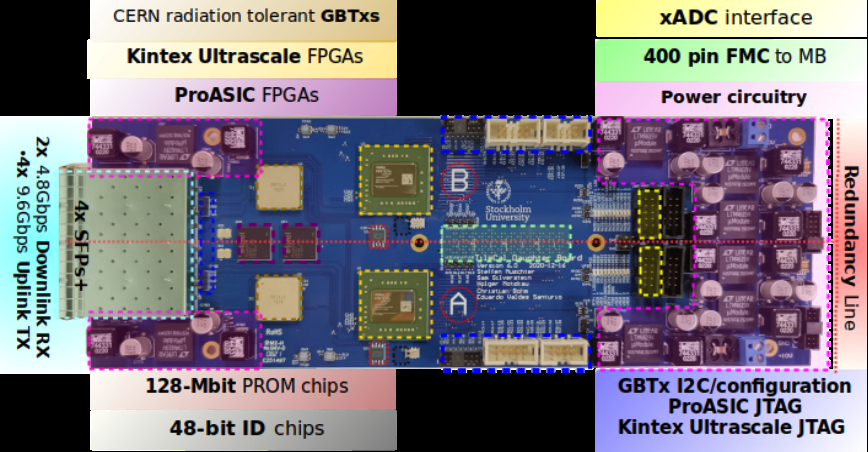
\includegraphics[width=0.8\linewidth]{assets/paper_ATL-TILECAL-PROC-2022-017_slide_3_item_1.png}
\end{figure}

Figure 2 .   The DB6 layout.

-- 2 --

\section*{Slide 4}

Two 20 nm planar featured Xilinx Kintex Ultrascale (KU) FPGAs distribute clocks and con- 
figuration received from the GBTx to the MB, while reading slow integrator data and fast digitized 
data   from   two   different   gains   of   the   PMTs.   The   xADCs   of   the   KU   FPGAs   sample   temperature, 
voltage stability and currents.   An over-current protection circuit triggers a power cycle in the case 
of the presence of high currents.   Each KU FPGA sends data off-detector by means of two copies of 
GBT-FEC protected words through two 9.6 Gbps uplinks.   The board radiation tolerance is achieved 
by   the   redundancy   layers   in   the   design,   using   the   Xilinx   Soft   Error   Management   (SEM),   Triple 
Mode Redundancy (TMR), GBT-FEC protocol, and GBTx ASICs.

4 
Radiation tests on the DB6

Four Daughterboards were separately used to test for radiation tolerance, labelled in this document 
as DB6-0, DB6-1, DB6-2 and DB6-3. 
Two   separate   tests   were   performed   to   cover   tolerance   to   Total   Ionizing   Dose   (TID).   The   KU 
FPGA   temperatures   and   all   the   currents   corresponding   to   all   the   point   of   load   regulators   of   the 
irradiated boards were monitored.   Special attention was placed on the total of ten Coretek SFP+, 
the   six   KU   FPGAs,   the   six   Microsemi   ProaSIC3   FPGAs   and   the   IS25LP128F   reconfiguration 
FLASH   memories.   None   of   the   components   were   damaged   by   the   deposited   TID:   DB6-1   and 
DB6-2   were   irradiated   with   Gamma   radiation   at   60 Co   at   the   CERN   CC60   facilities   to   220   Gy   at 
a   rate   of   3.37   Gy/h   (Figure   9   of   Ref.[ 4 ])   and   up   to   54   Gy   at   a   rate   of   0.33   Gy/h   (Figure   10   of 
Ref.   [ 4 ]),   respectively.   DB6-1   ran   stable   during   the   full   test,   however   it   showed   an   increase   in 
the   current   measured   in   the   0.95   V   power   line   of   both   sides   of   the   board   of   at   around   140   Gy. 
This   was   demonstrated   to   be   correlated   with   the   failure   of   the   active   components   of   the   fan   used 
to   keep   the   KU   FPGAs   cool,   leading   to   the   increase   of   temperature   on   the   FPGA.   The   currents, 
temperatures and functionalities of the DB6-2 were stable during the full run.   DB6-3 was irradiated 
in the AlC-144 cyclotron proton beam line with 54 MeV protons at the IFJ in Krakow to 381 Gy for 
half-A FPGA and 400 Gy for half-B FPGA at a rate of 2.88 Gy/h (Figure  3 ).   All the currents and 
the temperatures were stable during the full run.   The higher fluctuations compared with DB6-1 (0 
to 140 Gy) and DB6-2 are due to active Single Event Upset (SEU) corrections by the Xilinx SEM 
and resets applied when an uncorrectable SEU appeared during the run. 
Two separate tests were performed for Single Event Latchups (SEL), one as described for the 
DB6-3 with 54 MeV protons, where the FPGAs were irradiated to a fluence of 2.62  $\times$ 10 11   p/cm 2 .   In 
the second test, two Trenz TE0841 boards (each with the same KU FPGA used in the DB design), a 
Lattice ICE40LP FPGA and a ProASIC3E A3P31500 FPGA were irradiated with 226 MeV protons 
to a fluence of 1.11  $\times$ 10 12   p/cm 2 , for which all the currents of the FPGAs were monitored (Figure 
6 of Ref.   [ 4 ]).   No SEL were observed in the units under test in either of the tests. 
A set of tests was setup to cover the Non-Ionizing Energy Losses (NIEL) tolerance,   where a 
DB (DB6-0) and a set of test boards with non-radiation qualified DB components were irradiated 
to a fluence of 14  $\times$ 10 12   (1 MeV equivalent n)/cm 2 .   The post-radiation tests performed on DB6-0 
demonstrated   the   radiation   tolerance   of   the   KU   FPGAs   up   to   the   exposed   fluence.   In   the   case   of 
the ProASIC, some after-effects could be seen where the firmware was not working as expected and 
re-configuration was not possible.   However, the firmware functionality of all devices was recovered 
after annealing, with re-configuration capability recovered in some of the devices.   The same applies

-- 3 --

\section*{Slide 5}

\begin{figure}[H]
\centering
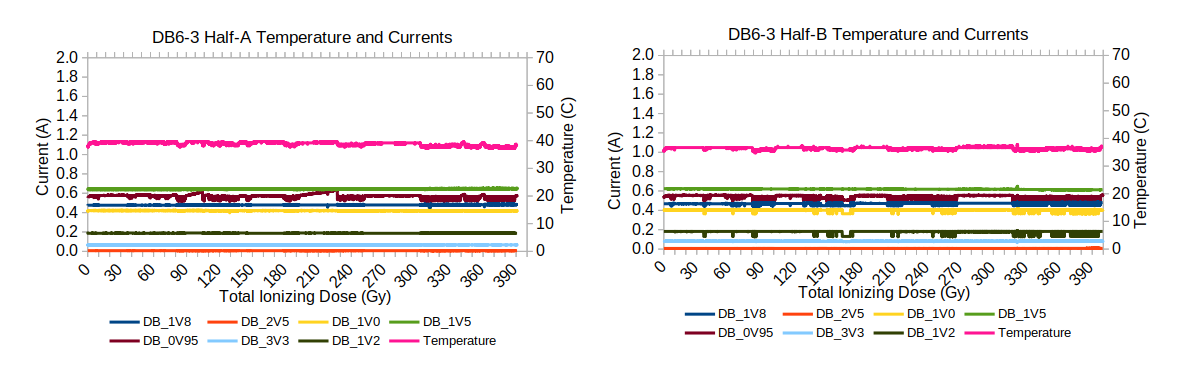
\includegraphics[width=0.8\linewidth]{assets/paper_ATL-TILECAL-PROC-2022-017_slide_5_item_1.png}
\end{figure}

Figure 3 .   TID test of DB6-3.   All board currents and the temperatures of both KU FPGAs were monitored 
over the whole irradiation period delivered by a 54 MeV proton beam.

to   the   IS25LP128F   FLASH   memories,   where   after   annealing   some   of   the   devices   recovered   the 
re-programing   capabilities,   with   all   the   contents   of   the   memory   not   being   affected   in   any   of   the 
devices.

Four different variants of 10 Gbps multi-mode SFP+ devices were tested:   AVAGO, CORETEK, 
FS-Europe   and   Direktronik.   The   two   AVAGO   AFBR-709SMZ   devices   completely   failed   to   pass 
the   irradiation   tests   done   up   to   9   $\times$ 10 12   (1   MeV   equivalent   n)/cm 2   fluence. 
One   out   of   nine 
CORETEK   CT-A000NPP-SB1L-D   devices   tested   failed   to   function   after   irradiating   to   9   $\times$ 10 12

(1   MeV   equivalent   n)/cm 2   fluence.   In   the   case   of   the   Direktronik   33-4248   and   the   FS-Europe 
SFP-10GSR-85 devices, one of each of the two brands was exposed to a higher fluence of 14 $\times$ 10 12

(1   MeV   equivalent   n)/cm 2 ,   and   a   batch   of   ten   of   each   of   the   two   brands   was   exposed   to   7   $\times$ 10 12

(1 MeV equivalent n)/cm 2   fluence.   All of the samples irradiated from Direktronik and FS-Europe 
were fully functional after irradiation.

It   was   seen   that   the   threshold   voltages   for   the   FDFMA3N109   MOSFETs   used   in   the   design 
shifted with the exposure (Figure  4 ) due to the Gamma component present in the reactor cavity (195 
Gy).   The asymmetrical profile of the flux in the cavity was used to have a perception of the correla- 
tion between the shifts of the thresholds in the MOSFETs and the exposed fluence.   Four out of fifteen

\begin{figure}[H]
\centering
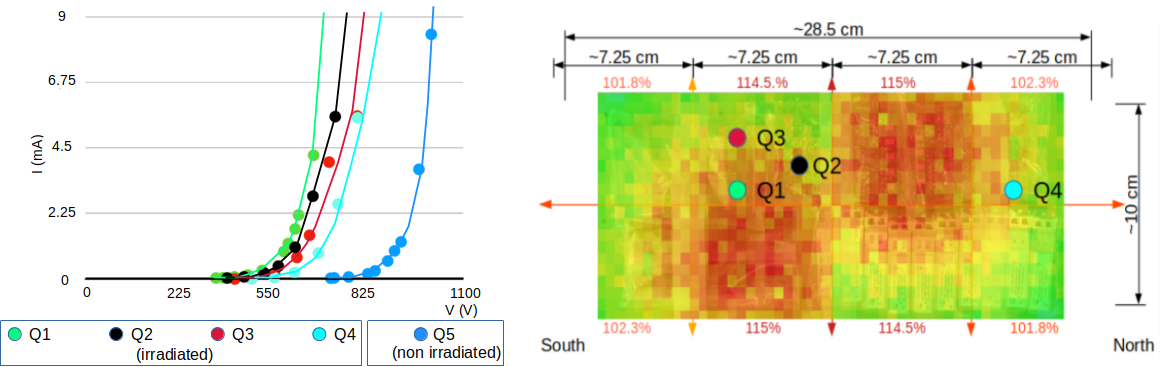
\includegraphics[width=0.8\linewidth]{assets/paper_ATL-TILECAL-PROC-2022-017_slide_5_item_2.png}
\end{figure}

Figure 4 .   (Left:)   Threshold shift depicted in an IV curve of four of the irradiated FDFMA3N109 MOSFETs. 
(Right:)   Position of the irradiated MOSFETs in the flux 2D slice map of the reactor cavity.

-- 4 --

\section*{Slide 6}

QUAD oscillators LTC6902IMS irradiated failed to pass the post irradiation tests, therefore the de- 
vice needs to be removed from the design.   The rest of the components (DAN217T146CT Schottky 
diodes, 540BAA100M000BBG oscillators and INA333AIDRG instrumentation amplifiers) passed 
the post radiation tests with no issues.

5 
Conclusions

Radiation test campaigns took place to qualify each of the components of the DB6 design to fulfill 
the   HL-LHC   requirements. 
The   outcome   of   the   tests   have   proved   that   the   design   is   TID   and 
SEL-resistant.   The   extra   protection   added   to   the   design   for   SEL   appearances   in   the   form   of   a 
over-current   circuit   has   to   be   removed   due   to   the   shift   in   the   threshold   of   the   MOSFETS   used   in 
the   implementation.   Similarly,   the   QUAD   oscillators   used   to   de-couple   the   phase   of   the   DC-DC 
converters   have   to   be   removed   from   the   design,   and   extra   studies   has   to   be   performed   to   assess 
the   impact   of   this   design   modification   on   the   board   noise.   The   removal   of   the   QUAD   oscillators 
and the over-current circuit will make the design sufficiently radiation-hard for the expected NIEL 
fluence of the full life of the HL-HLC. Future plans include producing extra prototypes that include 
the   aforementioned   modifications,   performing   Single   Event   Upset   tests,   and   following-up   in   the 
tests to finalize the selection of the SFP+ variant to be used with the final board design.   After the 
design is modified accordingly to the test results, prototypes will be produced and tested as part of 
the road map for the production phase of the project.   A total of 930 DB6 will be produced as the 
contribution of Stockholm University to the HL-LHC era for TileCal.

References

[1]   ATLAS Collaboration, 2008 JINST 3 S08003,

https://iopscience.iop.org/article/10.1088/1748-0221/3/08/S08003/pdf

[2]   ATLAS collaboration. Technical Design Report for the Phase-II Upgrade of the ATLAS Tile 
Calorimeter. CERN-LHCC-2017-019, ATLAS-TDR-028, 2018. 
https://cds.cern.ch/record/2285583

[3]   E. Valdes, 2019, Development of the read-out link and control board for the ATLAS Tile Calorimeter 
Upgrade, JACoW ICALEPCS2021 (2022) 290-296, ISBN: 978-91-7797-896-1, 
http://www.diva-portal.org/smash/get/diva2:1364842/FULLTEXT03.pdf

[4]   E. Valdes, S. Silverstein, C. Bohm, K. Dunne, S. Lee, R\&D Studies for the Atlas Tile Calorimeter 
Daughterboard, JACoW ICALEPCS2021 (2022) 290-296, DOI: 
10.18429/JACoW-ICALEPCS2021-TUAL03, 
https://inspirehep.net/files/5b1aad00535076acda8f14a848cc2d21

-- 5 --

\end{document}
